\part{Foundations}

\chapter{Probabilistic Circuits}
\label{chap:boolean_prob_circuits}

\section{Boolean Functions}
\label{sec:boolean_functions}

Let \(\mathbf{x} = (x_1, x_2, \dots, x_n)\) be a vector of \(n\) Boolean variables, where each \(x_i \in \{0,1\}\). A \emph{Boolean function} is a map
\begin{equation}
\label{eq:boolean_function}
F(\mathbf{x}) \;=\; F(x_1, x_2, \dots, x_n) \;\in\; \{0,1\}.
\end{equation}
This function takes each possible configuration of \(\mathbf{x}\) (i.e., each element of \(\{0,1\}^n\)) to a single binary output in~\(\{0,1\}\). Boolean functions appear throughout digital logic, circuit design, and a wide range of computational applications.

For illustration, we can visualize small Boolean functions based on the size of \(\mathbf{x}\). For \(n=1\), there are two possible input states:

\begin{center}
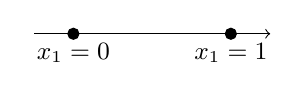
\begin{tikzpicture}
\filldraw[black] (0,0) circle (2pt) node[anchor=north]{\small $x_1=0$};
\filldraw[black] (2,0) circle (2pt) node[anchor=north]{\small $x_1=1$};
\draw[->] (-0.5,0) -- (2.5,0);
\end{tikzpicture}
\end{center}

For \(n=2\), the four possible states can be positioned on a 2D lattice:

\begin{center}
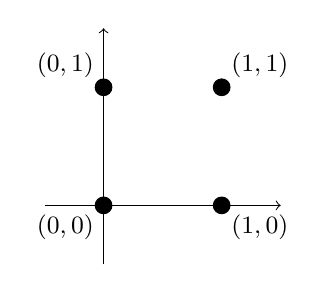
\begin{tikzpicture}[scale=1.5]
\filldraw[black] (0,0) circle (2pt) node[anchor=north east]{\small $(0,0)$};
\filldraw[black] (1,0) circle (2pt) node[anchor=north west]{\small $(1,0)$};
\filldraw[black] (0,1) circle (2pt) node[anchor=south east]{\small $(0,1)$};
\filldraw[black] (1,1) circle (2pt) node[anchor=south west]{\small $(1,1)$};
\draw[->] (-0.5,0) -- (1.5,0);
\draw[->] (0,-0.5) -- (0,1.5);
\end{tikzpicture}
\end{center}

In three dimensions (\(n=3\)), the eight possible states correspond to the vertices of a cube:

\begin{center}
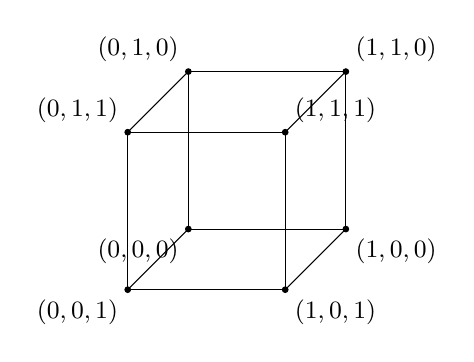
\begin{tikzpicture}[scale=2]
\coordinate (000) at (0,0,0);
\coordinate (001) at (0,0,1);
\coordinate (010) at (0,1,0);
\coordinate (011) at (0,1,1);
\coordinate (100) at (1,0,0);
\coordinate (101) at (1,0,1);
\coordinate (110) at (1,1,0);
\coordinate (111) at (1,1,1);

\foreach \point in {(000),(001),(010),(011),(100),(101),(110),(111)}
    \filldraw[black] \point circle (0.5pt);

\draw (000) -- (100) -- (110) -- (010) -- (000);
\draw (001) -- (101) -- (111) -- (011) -- (001);
\draw (000) -- (001);
\draw (100) -- (101);
\draw (110) -- (111);
\draw (010) -- (011);

\node[anchor=north east] at (000) {\small $(0,0,0)$};
\node[anchor=north west] at (100) {\small $(1,0,0)$};
\node[anchor=south east] at (010) {\small $(0,1,0)$};
\node[anchor=south west] at (110) {\small $(1,1,0)$};
\node[anchor=north east] at (001) {\small $(0,0,1)$};
\node[anchor=north west] at (101) {\small $(1,0,1)$};
\node[anchor=south east] at (011) {\small $(0,1,1)$};
\node[anchor=south west] at (111) {\small $(1,1,1)$};
\end{tikzpicture}
\end{center}

Boolean operators such as AND (\(\land\)), OR (\(\lor\)), and NOT (\(\lnot\)) allow constructing a wide variety of logical relationships. For example, in a setting where a system fails if any one of two components fails, the Boolean function can be written as
\[
F(x_A, x_B) \;=\; x_A \;\lor\; x_B.
\]
Here, \(F=1\) precisely when \(x_A=1\) or \(x_B=1\), encompassing a failure event if either component \(A\) or \(B\) is in state 1. More complex systems with many interdependent components may require Boolean functions with numerous variables and deeply nested operators.

Although Boolean functions are crucial for representing logical configurations, they operate purely in a binary framework and do not directly encode probability distributions. To include probabilistic behavior, we can move to a more expressive framework called \emph{probabilistic circuits}, which describe the distribution of variables in a directed acyclic graph (DAG). Such representations can capture both the combinatorial structure of system states and the uncertainty or likelihood associated with these states.

\section{Definition and Structure}

Consider a set of random variables \(\mathbf{X} = (X_1, X_2, \dots, X_n)\). A \emph{probabilistic circuit} \(\mathcal{C}\) is a DAG whose nodes consist of:

\begin{itemize}
 \item \textbf{Input nodes (leaves):} Each leaf encodes a base distribution over some subset of \(\mathbf{X}\). Often, these leaves correspond to univariate distributions \(p(X_i)\) or constant/indicator functions.
 \item \textbf{Internal nodes (gates):} Each gate combines incoming distributions from its children using either:
   \begin{itemize}
   \item \textbf{Sum-gates (mixture gates):} Weighted sums of child distributions, with nonnegative weights summing to 1.
   \item \textbf{Product-gates:} Factorized products of child distributions, each child covering disjoint subsets of \(\mathbf{X}\).
   \end{itemize}
\end{itemize}
The acyclic nature of the graph ensures that information flows consistently from the leaves toward a designated \emph{root} node.

\subsection{Sum-Gates and Product-Gates}

Let \(v\) be an internal node in \(\mathcal{C}\). Denote the children of \(v\) by \(\operatorname{ch}(v)\). Then:

\begin{itemize}
\item \textbf{Sum-gate:} Suppose \(v\) has children \(u_1,\dots,u_k\) with mixture weights \(\{\theta_{v,u_i}\}_{i=1}^k\) satisfying \(\sum_{i=1}^k \theta_{v,u_i} = 1\) and \(\theta_{v,u_i} \ge 0\). The distribution encoded at \(v\) is
\begin{equation}
\label{eq:sum_gate}
p_v(\mathbf{x}) \;=\; \sum_{i=1}^k \theta_{v,u_i}\,p_{u_i}(\mathbf{x}),
\end{equation}
where \(p_{u_i}(\mathbf{x})\) is the distribution encoded by child node \(u_i\).

\item \textbf{Product-gate:} Suppose \(v\) has children \(u_1,\dots,u_k\), each covering disjoint subsets of \(\mathbf{X}\). Let \(\mathbf{X}=\bigcup_{i=1}^k \mathbf{X}_{u_i}\) and \(\mathbf{X}_{u_i}\cap \mathbf{X}_{u_j} = \varnothing\) for \(i\neq j\). Then the distribution at \(v\) is
\begin{equation}
\label{eq:product_gate}
p_v(\mathbf{x})
\;=\;
\prod_{i=1}^k
p_{u_i}\bigl(\mathbf{x}_{u_i}\bigr),
\end{equation}
where \(\mathbf{x}_{u_i}\) is the restriction of \(\mathbf{x}\) to the variables in \(\mathbf{X}_{u_i}\).
\end{itemize}

\subsection{Leaf Nodes and the Circuit Distribution}

Each leaf node encodes a base distribution over its subset of variables (or a constant/indicator). Let \(v\) be a leaf node associated with \(p_v(\mathbf{X}_v)\). When the circuit is evaluated, each leaf contributes its assigned distribution or constant term. By recursively composing sum-gates and product-gates, every node \(v\) in the circuit defines a distribution \(p_v(\mathbf{x})\). The distribution of the entire circuit is given by evaluating its \emph{root} node \(r\):
\[
p_r(\mathbf{x}) \;=\; \text{(\(r\) evaluated from the leaves up)}.
\]

Probabilistic circuits unify structural and probabilistic modeling in a single formalism. They are widely used in fields such as artificial intelligence, machine learning, and automated reasoning, offering a tractable way to represent complex, high-dimensional probability distributions while preserving interpretable, compositional structure.


\chapter{Probabilistic Risk Assessment}

\section{The Triplet Definition of Risk}
\label{sec:triplet_definition_of_risk}
A central goal of risk analysis in nuclear engineering is to enable sound decision-making under large uncertainties. To achieve this, risk must be defined in a way that is both rigorous and practically quantifiable. One widely accepted definition, tracing back to seminal work in Refs.~\cite{kaplan_quantitative_1981}, frames risk as a \emph{set of triplets}. Each triplet captures three essential dimensions:

\begin{enumerate}
  \item \textit{What can go wrong?}
  \item \textit{How likely is it to happen?}
  \item \textit{What are the consequences if it does happen?}
\end{enumerate}

In more formal terms, let
\begin{equation}
\label{eq:risk_triplets}
    R \;=\;
    \bigl\{\,
        \langle
            S_i,\,
            L_i,\,
            X_i
        \rangle
    \bigr\}_{c}
\end{equation}
where \(R\) denotes the overall risk for a given system or activity, and the subscript \(c\) emphasizes \emph{completeness}: ideally, all important scenarios must be included. In this notation:
\begin{itemize}
    \item \(S_i\) specifies the \(i\)th \textbf{scenario}, describing something that can go wrong (e.g.\ an initiating event or equipment failure).  Typically, \(S_i \in \mathcal{S}\), where \(\mathcal{S}\) is the set of all possible scenarios.
    \item \(L_i\) (sometimes denoted \(p_i\) or \(\nu_i\)) is the \textbf{likelihood} (probability or frequency) associated with scenario~\(S_i\).  In other words, \(L_i\in [0,1]\) if modeled as a probability, or \(L_i\in [0,\infty)\) if modeled as a rate/frequency.
    \item \(X_i\) characterizes the \textbf{consequence}, i.e.\ the severity or nature of the outcome if the scenario occurs. Consequences can range from radiological releases and economic cost to broader societal impacts. In some analyses, \(X_i\) is a single-valued metric in \(\mathcal{X}\); in others, it may be treated as a distribution over possible outcomes in \(\mathcal{X}\).
\end{itemize}

The notation \(\{\cdot\}_{c}\) in Eq.~\eqref{eq:risk_triplets} stresses that \emph{all} substantial risk scenarios must be included. Omitting a significant scenario might severely underestimate total risk. One might ask, ``What are the uncertainties?'' In this dissertation, uncertainties are embedded in each \(L_i\) (and sometimes \(X_i\)) via probability distributions.

\subsection{Scenario Approach to PRA}
\label{sec:scenario_approach_to_pra}

A practical way to enumerate each triplet \(\langle S_i, L_i, X_i\rangle\) is through logical decomposition of potential failures or disruptions, a process referred to as \emph{scenario structuring}. Scenario structuring helps answer the question ``\textit{What can go wrong?}'' in greater detail by dividing possible scenarios into commonly recognized classes. Each of these categories corresponds to a distinct family of \emph{initiating events} (IE) that can trigger a chain of subsequent events or failures. At each node in the success scenario, we identify the IEs, which branch off from the initial success path \(S_0\) into new pathways that may lead to undesirable states. Thus, each \emph{scenario} \(S_i\) can be interpreted as a distinct departure from the baseline success path, triggered by some IE that occurs at node \(i\). From that point onward, a sequence of \emph{conditional events} or barriers may succeed or fail, culminating in an end-state \(ES_i\).

\section{Definition of an Event Tree}
\label{sec:event_tree_definition}

Event trees unravel how a single \emph{initiating event} (\(I\)) can branch into multiple possible \emph{end-states} (\(X\)) through a sequence of \emph{functional} (or conditional) events. Each branch captures the success or failure of an important \emph{functional event} (e.g.\ a safety barrier or operator intervention). By following all possible paths, one can systematically account for each final outcome \(X_j\). Figure~\ref{fig:event_tree_example} provides a schematic view of this process for an initiating event \(I\) and two subsequent functional events, \(F_1\) and \(F_2\). Each terminal node (leaf) corresponds to a distinct end-state, denoted \(X_1, X_2, \ldots, X_n\). Though this illustration is intentionally simple, more complex systems may include numerous functional events, each branching into further outcomes.

\begin{figure}[ht!]
\centering

\begin{tikzpicture}
\tikzset{grow'=right,level distance=48pt}
\tikzset{execute at begin node=\strut}
\tikzset{every tree node/.style={anchor=base west}}
\tikzset{
    edge from parent/.append style={very thick},
    edge from parent/.style={
        draw,
        edge from parent path={
            (\tikzparentnode.east) -| ($(\tikzparentnode.east)!0.5!(\tikzchildnode.west)$) |- (\tikzchildnode.west)
        },
    },
    every node/.style={anchor=center,font=\small\bfseries, text centered, inner sep=0pt},
    every level 0 node/.style={circle, font=\small\bfseries, draw, fill=blue!30, inner sep=0pt},
    every internal node/.style={font=\small, inner sep=4pt},
    every leaf node/.style={rectangle, draw, fill=blue!30, minimum width=2.5cm, text centered},
    frontier/.style={distance from root=400pt},
}
\Tree [.\(I\)
    [.\(F_1^{\text{succ}}\)
        [.\(F_2^{\text{succ}}\)
            [.\(X_1\) ]
        ]
        [.\(F_2^{\text{fail}}\)
            [.\(X_2\) ]
        ]
    ]
    [.\(F_1^{\text{fail}}\)
        [.\(X_3\) ]
    ]
]
\end{tikzpicture}
\caption{Illustrative event tree with an initiating event \(I\), two functional events \(F_1\) and \(F_2\), and three end-states \(X_1, X_2, X_3\).}
\label{fig:event_tree_example}
\end{figure}

At the highest conceptual level, an event tree is a collection of conditional outcomes. Let \(n\) be a positive integer, and let \(j\) range over some index set of end-states~\(J\). Then define
\begin{equation}
\label{eq:event_tree_gamma}
    \Gamma
    \;=\;
    \Bigl\{
        \langle
            I,\,
            F_1,\,
            F_2,\,
            \dots,\,
            F_n,\,
            X_j
        \rangle
        :\,
        j \in J
    \Bigr\},
\end{equation}
where:
\begin{itemize}
    \item \(I\) is the \textbf{initiating event}. In a nuclear system, this could be an abnormal occurrence such as a coolant pump trip or an unplanned reactivity insertion.
    \item \(F_k\) (\(k=1,\ldots,n\)) denotes the \(k\)th \textbf{functional (conditional) event}, which may succeed (\(F_k^{\text{succ}}\)) or fail (\(F_k^{\text{fail}}\)). Typically, each \(F_k\) depends on the outcomes \(F_1,\ldots,F_{k-1}\).
    \item \(X_j\) is an \textbf{end-state}, describing the final outcome along a particular branch. End-states might indicate safe shutdown, core damage, or a radiological release.
\end{itemize}
Each tuple \(\langle I, F_1, \dots, F_n, X_j\rangle\) in \(\Gamma\) encapsulates a distinct scenario pathway. In the broader context of the risk triplet, such a pathway corresponds to \(S_i\), the possibility of something going wrong, while the associated probability and consequences map directly to \(L_i\) and \(X_i\).

\subsection{Probabilistic Representation}

Because risk analysis requires knowing how likely each branch in the tree is, event trees rely heavily on \emph{conditional probabilities}. Let
\[
    p(I)
    \;\equiv\;
    \Pr(I)
\]
be the probability (or frequency) of the initiating event. For each functional event \(F_k\), define
\[
    p\bigl(F_k^{\text{succ}}\mid I,\, F_1,\,\dots,\,F_{k-1}\bigr)
    \quad\text{and}\quad
    p\bigl(F_k^{\text{fail}}\mid I,\, F_1,\,\dots,\,F_{k-1}\bigr),
\]
which describe the likelihood of success or failure given all prior outcomes.

An \emph{end-state} \(X_j\) arises from a particular chain of successes/failures:
\[
    \bigl(I,\,F_1^{\alpha_1},\,F_2^{\alpha_2},\,\ldots,\,F_n^{\alpha_n}\bigr)
    \;\longrightarrow\; 
    X_j,
\]
where each \(\alpha_k \in \{\text{succ},\,\text{fail}\}\). The probability of reaching \(X_j\) is the product of:
\begin{enumerate}
    \item The initiating event probability \(p(I)\).
    \item The conditional probabilities of each functional event's success or failure.
\end{enumerate}
Formally, if \(\omega_j\) denotes the entire branch leading to end-state \(X_j\), then
\begin{align}
\label{eq:event_tree_branch_probability}
    p(\omega_j)
    \;=\;
    p(I)
    \times
    \prod_{k=1}^{n}\,
    p\!\bigl(F_k^{\alpha_k}\mid 
             I,\,
             F_1^{\alpha_1},\ldots,
             F_{k-1}^{\alpha_{k-1}}\bigr).
\end{align}
The union of all such branches spans the full sample space of scenario outcomes generated by \(I\) and the subordinate functional events. Next, we show that every branch of an event tree can be represented by a product (logical AND) of the relevant Boolean variables for the initiating event and each functional event’s success/failure.  Collecting all branches via logical OR yields a disjunction of these products, precisely matching the standard structure of a Boolean expression in disjunctive normal form (DNF).

\subsection{Event Tree Structures as Sum-Product Networks}
Consider a specific branch \(\omega_j\) leading to the end-state \(X_j\).  By definition, \(\omega_j\) occurs if and only if:
\begin{enumerate}
    \item The initiating event \(I\) happens: \(i=1\).
    \item For each functional event \(F_k\), the branch specifies a particular outcome (success or failure).  Suppose \(\omega_j\) includes successes for some subset of indices \(\alpha\subseteq \{1,\ldots,n\}\) and failures for the complementary indices.  We can write this as:
    \[
        \bigwedge_{k\in \alpha}  \bigl(f_{k}^{\text{succ}} = 1\bigr)
        \quad\wedge\quad
        \bigwedge_{k\notin \alpha} \bigl(f_{k}^{\text{fail}} = 1\bigr).
    \]
\end{enumerate}
Hence, the branch event \(\omega_j\) is logically equivalent to a single \emph{product term}:
\begin{equation}
\label{eq:branch_conjunction}
    \omega_j \;\equiv\; 
    \bigl(i=1\bigr)
    \;\wedge\;
    \bigwedge_{k\in \alpha} \bigl(f_k^{\text{succ}}=1\bigr)
    \;\wedge\;
    \bigwedge_{k\notin \alpha} \bigl(f_k^{\text{fail}}=1\bigr).
\end{equation}
In standard Boolean notation, each literal (e.g., \(f_k^{\text{succ}}\)) is a variable that can be 0 or 1, and the branch is the \(\land\) (AND) of those variables. An event tree describing all possible outcomes from \(I\) and the subsequent functional events can be viewed as the union (logical OR) of its disjoint branches:
\[
    \Omega \;=\; \omega_1 \;\cup\; \omega_2 \;\cup\;\cdots \;\cup\; \omega_m.
\]
In Boolean terms, this is the \(\lor\) (OR) of the product terms corresponding to each branch:
\begin{equation}
\label{eq:event_tree_disjunction}
    \Omega
    \;\equiv\;
    \omega_1
    \;\lor\;
    \omega_2
    \;\lor\;\cdots\lor\;
    \omega_m.
\end{equation}
Substituting each branch’s conjunction form (as in Eq.~\eqref{eq:branch_conjunction}) into Eq.~\eqref{eq:event_tree_disjunction} yields:
\[
    \Omega 
    \;\;=\;\;
    \Bigl[
        i \;\wedge\; \prod_{k\in \alpha_1} f_k^{\text{succ}} \;\wedge\; \prod_{k\notin \alpha_1} f_k^{\text{fail}}
    \Bigr]
    \;\;\lor\;\;
    \Bigl[
        i \;\wedge\; \prod_{k\in \alpha_2} f_k^{\text{succ}} \;\wedge\; \prod_{k\notin \alpha_2} f_k^{\text{fail}}
    \Bigr]
    \;\;\lor\;\;
    \cdots
\]
where each \(\alpha_r\) is the set of functional events that succeed along branch \(r\).

A standard DNF (sum-of-products) expression in Boolean algebra is
\[
    \bigl(\text{literal}_1 \;\wedge\;\text{literal}_2 \;\wedge\;\cdots\bigr)
    \;\;\lor\;\;
    \bigl(\text{literal}_{1}' \;\wedge\;\text{literal}_{2}' \;\wedge\;\cdots\bigr)
    \;\;\lor\;\;\cdots
\]
Each term in the sum (OR) is a logical AND of literals (variables or their negations). Comparing with Eq.~\eqref{eq:event_tree_disjunction}, we see that an event tree is exactly a disjunction of terms, each term being a conjunction of the initiating event \(i\) (set to 1) and the success/failure indicators for each \(F_k\). Since any negation can be encoded by stating whether \(F_k\) is \(\text{succ}\) (\(f_k^{\text{succ}}=1\)) or \(\text{fail}\) (\(f_k^{\text{fail}}=1\)), the entire event tree \(\Omega\) is in DNF:
\[
    \Omega \;=\; 
    \bigvee_{j=1}^m
    \Bigl[
        \;\bigwedge_{\ell\in \Lambda_j}
        (\text{appropriate literal})
    \Bigr].
\]

\subsection{Expressivity and Tractability of Event Trees}
\label{sec:tractability_event_trees}

Within \(\operatorname{SP}\!-\)networks (sum-product networks), a sum gate provides a weighted sum of child distributions, whereas a product gate factorizes them.  An event tree can be cast as an \(\operatorname{SP}\!-\)network by feeding each branch’s literal probabilities into product gates (one per branch), then summing over all branches with a sum gate.  Once constructed, evaluating the resulting \(\operatorname{SP}\!-\)network at a specific configuration \(\mathbf{x}\) or marginalizing out some of the variables is linear in the size of that network.  Nevertheless, the tractability of event trees (and their circuit representations) heavily depends on their size and structure.  We summarize several key considerations below:

\begin{enumerate}
    \item \emph{DNF size grows exponentially.}
    
    Suppose an event tree includes \(n\) functional events, each of which can succeed or fail.  In the worst case, enumerating \emph{all} possible outcome branches (i.e.\ each success/failure pattern) yields up to \(2^n\) conjunction terms.  Hence, the disjunctive normal form (DNF) representation can become exponentially large.  Computing or marginalizing probabilities over such a large DNF may become prohibitively expensive if \(n\) is large enough.

    \item \emph{Evaluation linear in network size.}
    
    Even though the DNF itself may blow up exponentially, once the event tree is translated into an \(\operatorname{SP}\!-\)network, key inference tasks (such as evaluating it at a configuration or marginalizing over certain variables) proceed in time linear in the \emph{compiled network size}.  That said, if the underlying network has already reached exponential size in the number of events, the linear-time evaluation does not necessarily improve the overall worst-case complexity.
    
    \item \emph{Approximations abound.}
    
    In practice, analysts often employ approximations to keep event trees tractable.  One possibility is \emph{decomposability}, a core principle behind tractable probabilistic circuits whereby each product gate operates on disjoint sets of variables.  If the system decomposes (e.g.\ different safety barriers protect disjoint sets of equipment), one can evaluate probabilities without enumerating all branches.  Another common approximation is to prune paths with very low probabilities or ignore paths that only negligiblly contribute to the overall risk.
\end{enumerate}

Fully enumerated event trees, regardless of being interpretable as DNF/SP networks, trade tractability for expressivity. The intuitive branching structure and conditional probability assignments make event trees easy to interpret. PRA analysts can read off and reason about the high-level scenario decomposition, incorporate domain knowledge, and analyze each branch explicitly.  If the number of critical functional events is moderate, enumerating all branches remains tractable. As the depth and breadth of the tree grow, any brute-force probability computation over such a large DNF/SOP circuit is equally exponential in the worst case. Even though \(\operatorname{SP}\!-\)networks offer efficient linear-time evaluation with respect to the circuit size, the underlying circuit itself may have size exponential in \(n\).
\section{Definition of a Fault Tree}
\label{sec:fault_tree_definition}

% TODO: citep : Ruijters and Stoelinga - 2015 - Fault tree analysis A survey of the state-of-the-.pdf
Whereas \emph{event trees} begin with an initiating event and branch forward through possible outcomes, \emph{fault trees} (FT) are a top-down representation of how a specific high-level failure can arise from malfunctions in the components or subsystems of an engineered system. It is typically drawn as a tree or a DAG whose unique root node is the top event and whose leaves/basic events capture individual component failures or other fundamental causes. This hierarchical decomposition proceeds until all relevant failure modes are captured in the leaves or else grouped as undeveloped events.

\subsection{Nodes in a Fault Tree: Events and Gates}

Formally, the nodes of a fault tree can be divided into two main categories:  
\begin{itemize}
  \item \textbf{Events}, which denote occurrences at different hierarchical levels.  
    \begin{itemize}
      \item \emph{Basic events} (BEs) represent the lowest-level failures, typically single-component malfunctions or individual human errors. They are often depicted as circles or diamonds in diagrams.  
      \item \emph{Intermediate events} indicate the outcome of one or more lower-level events. Though intermediate events do not change the logical structure of the FT analysis, they can greatly enhance clarity by grouping sub-failures into a meaningful subsystem label (e.g., Cooling subsystem fails). They are typically drawn as rectangles.  
      \item \emph{Top event} (TE) is a single node, unique in the tree, that represents the high-level failure of interest (e.g., System fails).
    \end{itemize}
  \item \textbf{Gates}, which describe how events combine to produce a higher-level event. Each gate outputs a single event (often an intermediate or the top event), based on one or more input events.  
\end{itemize}

Because a fault tree traces failures up toward the top event, the overall structure becomes a DAG. If a particular event (basic or intermediate) is relevant to multiple subsystems, it can be shared among the inputs of different gates. Consequently, while many small FTs have a pure tree shape, large or intricate systems generally produce shared subtrees, yielding a more general DAG.

\subsection{Common Gate Types in Fault Trees}

FTs often use only a few canonical gate types (Figure~\ref{fig:gates}), each describing a logical relationship among its inputs:

\begin{itemize}
\item \textbf{AND gate} – The output event occurs only if \emph{all} input events occur.  
\[
  \text{Output} \;=\; e_1 \;\land\; e_2 \;\land\;\dots\;\land\; e_k.
\]
\item \textbf{OR gate} – The output event occurs if \emph{any} input event occurs.  
\[
  \text{Output} \;=\; e_1 \;\lor\; e_2 \;\lor\;\dots\;\lor\; e_k.
\]
\item \textbf{\(k\)-out-of-\(n\) gate (Voting gate)} – The output event occurs if \emph{at least} \(k\) of the \(n\) inputs fail. Denoted \(\mathrm{VOT}(k/n)\), it can be expressed by a large OR of all possible subsets of size \(k\), though notationally keeping it as one gate is much more concise.  
\[
  \text{Output} \;=\;
  \Bigl[\!\sum_{i=1}^n e_i \,\ge\, k\Bigr].
\]
\item \textbf{INHIBIT gate} – The output event occurs if a specific trigger event happens \emph{and} an additional conditioning event is present (often a privilege or a rarely active subsystem). This gate acts logically like an AND gate on two inputs, but is sometimes drawn differently for clarity.
\end{itemize}

\begin{figure}[h]
\centering
\begin{tikzpicture}[node distance=1.5cm,>=stealth,scale=0.85, every node/.style={scale=0.85}]

% AND gate
\node[draw, thick, minimum width=1cm, minimum height=1cm] (AND) {AND};
\node[above left=0.3cm and 0.35cm of AND] (ANDin1) {$e_1$};
\node[below left=0.3cm and 0.35cm of AND] (ANDin2) {$e_2$};
\draw[->, thick] (ANDin1) -- (AND.west);
\draw[->, thick] (ANDin2) -- (AND.west);
\node[right=0.7cm of AND] (ANDout) {Output};
\draw[->, thick] (AND.east) -- (ANDout);

% OR gate
\node[draw, thick, minimum width=1cm, minimum height=1cm, right=2.2cm of AND] (OR) {OR};
\node[above left=0.3cm and 0.35cm of OR] (ORin1) {$e_1$};
\node[below left=0.3cm and 0.35cm of OR] (ORin2) {$e_2$};
\draw[->, thick] (ORin1) -- (OR.west);
\draw[->, thick] (ORin2) -- (OR.west);
\node[right=0.7cm of OR] (ORout) {Output};
\draw[->, thick] (OR.east) -- (ORout);

% k of n gate
\node[draw, thick, minimum width=1.2cm, minimum height=1cm, right=2.2cm of OR] (VOT) {$k/n$};
\node[above left=0.3cm and 0.4cm of VOT] (VOTin1) {$e_1$};
\node[left=0.3cm of VOT] (VOTin2) {$\vdots$};
\node[below left=0.3cm and 0.4cm of VOT] (VOTin3) {$e_n$};
\draw[->, thick] (VOTin1) -- (VOT.west);
\draw[->, thick] (VOTin2) -- (VOT.west);
\draw[->, thick] (VOTin3) -- (VOT.west);
\node[right=0.7cm of VOT] (VOTout) {Output};
\draw[->, thick] (VOT.east) -- (VOTout);

\end{tikzpicture}
\caption{Examples of standard gate types in a fault tree: AND, OR, and \(k/n\) (voting).}
\label{fig:gates}
\end{figure}

If a system is large, detailed modeling of every component may not be warranted. In such cases, one may simplify certain subsystems by treating their failures as single \emph{undeveloped events}. An undeveloped event is effectively a basic event for analysis purposes, even though it may internally comprise several components. This method conserves complexity where the subsystem is either of negligible importance or insufficiently characterized to break down further.

A convenient formalization treats an FT as a structure \(F = \langle \mathcal{B}, \mathcal{G}, T, I \rangle\) where the unique top event \(t\) belongs to \(\mathcal{G}\), and:

\begin{itemize}
\item \(\mathcal{B}\) is the set of basic events. 
\item \(\mathcal{G}\) is the set of gates or internal nodes.
\item \(T: \mathcal{G} \to \text{GateTypes}\) assigns a gate type (AND, OR, \(k/n\), etc.) to each gate in \(\mathcal{G}\).  
\item \(I: \mathcal{G} \to \mathcal{P}(\mathcal{B} \cup \mathcal{G})\) specifies the input set of each gate, i.e.\ which events (basic or intermediate) feed into that gate.  
\end{itemize}

The graph is \emph{acyclic} and has a unique root (the top event \(t\)) that is reachable from all other nodes. If an element is the input to multiple gates, it may be drawn once and connected multiple times or duplicated visually; either way, the logical semantics remain the same.

\subsection{Fault Tree Semantics}

To interpret a fault tree, we examine which higher-level events fail when a subset \(S\) of basic events have failed. Denote by \(\pi_F(S, e)\) the \emph{failure state} (0 or 1) of element \(e\) given a set \(S\subseteq \mathcal{B}\) of failed basic events. Then:

\begin{itemize}
\item For each basic event \(b \in \mathcal{B}\):
  \[
    \pi_F(S, b) \;=\;
    \begin{cases}
      1, & b \in S,\\
      0, & b \notin S.
    \end{cases}
  \]
\item For each gate \(g \in \mathcal{G}\) with inputs \(\{x_1,\dots,x_k\}\subseteq \mathcal{B}\cup\mathcal{G}\):
  \[
  \pi_F(S,g) 
  \;=\;
  \begin{cases}
  \displaystyle
    \bigwedge_{i=1}^k \pi_F(S, x_i),
    & \;\text{if }T(g)=\mathrm{AND},\\[1.2em]
  \displaystyle
    \bigvee_{i=1}^k \pi_F(S, x_i),
    & \;\text{if }T(g)=\mathrm{OR},\\[1.2em]
  \displaystyle
    1 \;-\; \pi_F(S, x_1),
    & \;\text{if }T(g)=\mathrm{NOT} \text{ (single input)},\\[1.2em]
  \displaystyle
    \sum_{i=1}^k \pi_F(S,x_i)\;\ge\;k,
    & \;\text{if }T(g)=\mathrm{VOT}(k/n),\\
  \displaystyle
    \Bigl(\sum_{i=1}^k \pi_F(S,x_i)\Bigr)\bmod 2,
    & \;\text{if }T(g)=\mathrm{XOR} ,\\[0.6em]
  \end{cases}
  \]
\end{itemize}
The top event \(t\) (i.e., \(\mathrm{TE}\)) is a gate in \(\mathcal{G}\); we often write simply \(\pi_F(S)\) to mean whether the top event fails under the set \(S\) of failed BEs.

\subsubsection{Coherent vs. Noncoherent Fault Trees}
FTs are usually \emph{coherent}, meaning if a certain set of basic events causes a failure, then having more basic events fail cannot fix that failure—no NOT gates or other negations exist to undo the top event. However, some advanced FTs allow thresholds or special conditions that introduce partial noncoherence (e.g., a system that can fail only if a valve is stuck \emph{open} and a pump is \emph{working} to overpressurize a vessel). Such cases add complexity and require extended gates or additional modeling logic.

\subsection{Combining Shared Subtrees and Large Systems}

In standard reliability analysis, certain fault tree computations—such as identifying \emph{minimal cut sets} or calculating the probability of the top event—can be done by enumerating combinations of basic events that ensure system failure. However, if large shared subtrees exist or many gates gather multiple inputs, the expansion can become combinatorially challenging. Nevertheless, the DAG structure remains powerful for:

\begin{itemize}
\item \textbf{Clarity and Modularity:} Decomposing the system or subsystem failures into smaller, well-defined parts.  
\item \textbf{Reuse of Subtrees:} Representing components or subsystems that are relevant to multiple parts of the fault logic without arbitrarily duplicating them.  
\item \textbf{Analytical Efficiency:} Exploiting independence or bounding certain events, thereby limiting the combinatorial explosion.  
\end{itemize}

\subsection{Quantitative Analysis and Probability Estimation}
\label{sec:fault_tree_probability_estimation}

Beyond describing which combinations of basic events can fail, most fault tree analyses (FTAs) require a quantitative assessment of the \emph{likelihood} that the top event \(t\) ultimately occurs. This section details how to embed probabilities within the fault tree structure, how to compute the top event’s failure probability (or system \emph{unreliability}), and some common methods for handling large or dependent fault trees.

\subsubsection{Assigning Probabilities to Basic Events}

Let \(\mathcal{B}=\{b_1, \dots, b_n\}\) be the set of basic events in the fault tree \(F\).  Each basic event \(b\) is associated with a \emph{failure probability} \(p(b)\in [0,1]\).  Interpreted as a Boolean random variable \(X_b\), event \(b\) takes value \(1\) (failure) with probability \(p(b)\) and value \(0\) (success) with probability \(1-p(b)\).  Thus, 
\[
\Pr\bigl[X_b = 1\bigr] \;=\; p(b), 
\quad
\Pr\bigl[X_b = 0\bigr] \;=\; 1-p(b).
\]

In the simplest \emph{single-time} analysis, each basic event is either failed or functioning for the entire time horizon under study, and no component recovers once it has failed.

\subsubsection{Top Event Probability Under Independence}

If we assume that all basic events fail independently, then for any set \(S \subseteq \mathcal{B}\) of failed basic events,
\[
\Pr\bigl[\text{basic events in }S\text{ fail and others succeed}\bigr]
\;=\;
\prod_{b \in S} p(b)\,\times\!\!\prod_{b \notin S} [1 - p(b)].
\]
Recall from Section~\ref{sec:fault_tree_definition} that the top event \(t\) (also called \(\mathrm{TE}\)) fails given \(S\) precisely if \(\pi_F(S, t)=1\).  Hence, the probability that the top event fails is the sum of these independent configurations \(S\) for which \(\pi_F(S,t)=1\):
\begin{equation}
\label{eq:top_event_probability}
\Pr\bigl[X_t=1\bigr]
\;=\;
\sum_{S\,\subseteq\,\mathcal{B}}
\Bigl[
    \pi_F(S,t)
    \prod_{b \in S} p(b)
    \prod_{b \notin S} \bigl[1 - p(b)\bigr]
\Bigr].
\end{equation}
A direct computation of \eqref{eq:top_event_probability} often becomes unwieldy for large FTs because of the exponential number of subsets \(S\).  However, if the fault tree is \emph{simple} (no shared subtrees) and each gate in \(\mathcal{G}\) has independent inputs, one may propagate probabilities \emph{bottom-up} through the DAG using basic probability rules:
\[
\begin{aligned}
\Pr[g=1] \;=\;& \prod_{x \in I(g)} \Pr[x=1],
&&\text{if gate \(g\) is AND,}\\[6pt]
\Pr[g=1] \;=\;& 1 \;-\; \prod_{x \in I(g)}\bigl[1-\Pr[x=1]\bigr],
&&\text{if gate \(g\) is OR,}\\[6pt]
\Pr[g=1] \;=\;& 1 \;-\; \Pr[x=1],
&&\text{if gate \(g\) is NOT (single input \(x\)),}\\[6pt]
\Pr[g=1] \;=\;& \displaystyle \sum_{j=k}^{\,|I(g)|}
\;\;\sum_{\substack{A\,\subseteq\,I(g)\\|A|=j}}
\;\;\prod_{x\in A}\Pr[x=1]\;\prod_{x\in I(g)\setminus A}\bigl[1-\Pr[x=1]\bigr],
&&\text{if gate \(g\) is \(\mathrm{VOT}(k/n)\),}\\[6pt]
\Pr[g=1] \;=\;& \displaystyle \sum_{\substack{A\,\subseteq\,I(g)\\\text{\(|A|\) is odd}}}
\;\;\prod_{x\in A}\Pr[x=1]\;\prod_{x\in I(g)\setminus A}\bigl[1-\Pr[x=1]\bigr],
&&\text{if gate \(g\) is XOR.}
\end{aligned}
\]
\subsubsection{Dependence and Shared Subtrees}
In many real-world fault trees, a single basic event \(b\) may feed into multiple gates, thereby making different branches of the tree dependent on one another. This violates the independence assumptions that simple bottom-up probability propagation requires. Below, we list several techniques that address or approximate these dependencies:

\begin{enumerate}

  \item \textbf{Binary Decision Diagrams (BDDs).}  
  Using BDDs involves encoding the entire Boolean structure of the fault tree into a single, canonical DAG.  Sub-expressions within this diagram are cached, allowing an efficient evaluation of \(\Pr[X_t=1]\) even when basic events are shared across subtrees.  In many cases, BDDs compress large FTs and facilitate fast reliability inference.

  \item \textbf{Minimal Cut Sets (MCSs) and Approximations.}  
  Many approaches characterize the top event in terms of its minimal cut sets.  Let \(\{\mathrm{MCS}\}\) be the family of all minimal cut sets for the top event \(t\).  Each MCS \(C\subseteq \mathcal{B}\) is a smallest set of basic events whose simultaneous failure brings down the system.  

  \begin{itemize}
    \item \emph{Rare-Event Approximation.}  
    When each \(p(b)\) is small, the probability of two or more cut sets overlapping in their failures can be negligible.  A common approximation is to sum the probabilities of each MCS as if they were mutually exclusive:
    \begin{equation}\label{eq:rare_event_approx}
      \Pr[X_t=1]
      \;\approx\;
      \sum_{C\in \{\mathrm{MCS}\}}
      \;\prod_{b \in C} p(b).
    \end{equation}
    In highly reliable systems, this often yields a reasonable estimate.

    \item \emph{Min-Cut Upper Bound (MCUB).}  
    A related bounding technique interprets the top event as the union of all MCS failures. By the union bound,
    \begin{equation}\label{eq:mcub}
      \Pr[X_t=1]
      \;\le\;
      \sum_{C\in \{\mathrm{MCS}\}}
      \;\prod_{b \in C} p(b).
    \end{equation}
    Known as the \emph{min-cut upper bound}, this provides a guaranteed upper estimate for the probability of system failure.  However, if multiple MCSs share common basic events of non-negligible failure probability, one might overestimate \(\Pr[X_t=1]\).  
  \end{itemize}

  \item \textbf{Simulation-Based Methods.}  
  Monte Carlo simulation bypasses many analytical complexities by directly sampling the failure state of each basic event from its distribution \(p(b)\).  After sampling, one evaluates the fault tree deterministically (i.e., checks whether \(X_t=1\)).  Repeating over many samples yields an empirical estimate of the top event probability.  This approach is flexible, handles various dependencies, and easily extends to time-dependent or multi-state analyses.  However, for extremely rare failures, simulation can require large sample sizes to achieve low-variance estimates.

\end{enumerate}

Each of these techniques accommodates shared subtrees more effectively than naive bottom-up methods.  In practice, analysts often deploy a combination of them (e.g., using BDDs for certain gates, applying an MCS approximation for others) to balance accuracy, computational cost, and modeling complexity.


\usetikzlibrary {intersections}
\usetikzlibrary {graphs}
\begin{figure}[ht!]
\centering
\begin{tikzpicture}[domain=-4:12]
  % \draw [help lines] (-4,0) grid (12,12);
  \draw[->] (-4.0,0) -- (11,0) node[right] {$x$};
  \draw[->] (-4,0) -- (-4,12.0) node[above] {$f(x)$};
\begin{scope}[every node/.style={thick}]
    \node (ss_begin) at (-2.75,1.75) {$\text{S}_0$};

    \node (ss_end) at (9.5,11.0) {$\text{ES}_{0}$} ;
    % \node (ss_1) at (2.5,0.0) {$S_1$};
    % \node (ss_i) at (5.0,0.0) {$S_i$};
    % \node (ss_j) at (10.0,0.0) {$S_j$};
    % \node (ss_jp1) at (12.5,0.0) {$S_{j+1}$};

\end{scope}

\begin{scope}[>={Circle[black]},
              every edge/.style={draw=black,very thick}]
    % \path [->] (ss_0) edge (ss_1);
    % \path [->] (ss_1) edge (ss_i);
    % \path [->] (ss_i) edge (ss_j);
    % \path [->] (ss_j) edge (ss_jp1);
    % \path [->] (ss_jp1) edge (ss_f);
    % %\path [->] (B) edge node {$3$} (C);
    %\path [<->] (ss_begin) edge[out=25,in=220] node {} (ss_ie_i); 
    \path[<->,save path=\pathA,name path=A] (ss_begin) to [out=45,in=160, edge node={node [near end, above] {$\text{S}_0$}}](ss_end);

    \path[<->,save path=\pathB,name path=B] (1,0) to (1,11);

  \fill[name intersections={of=A and B}] (intersection-1) circle (3pt);

  \node[anchor=south east] (ss_ie_i) at (intersection-1) {$\text{IE}_i$};

  \draw[<->,black,very thick][use path=\pathA];
  %\draw[red] [use path=\pathB];
    %\path [<->] (ss_begin) edge[out=25,in=180] node[near end, above] {$\text{S}_0$} (ss_end); 
    %\path [<->] (ss_ie_i) edge[out=0,in=180] node[sloped] {} (ss_end); 
\end{scope}
\begin{scope}
  [grow'=right,
   level distance=50pt,
   every tree node/.append style={anchor=base west},
   execute at begin node=\strut,
   level 0/.style={sibling distance=0pt},  % initiating event
   level 1/.style={sibling distance=55pt}, %
   level 2/.style={sibling distance=45pt},
   level 3/.style={sibling distance=25pt, nodes={right=2}},
   edge from parent/.append style={
        draw,
        edge from parent path={
            (\tikzparentnode.east) -| ($(\tikzparentnode.east)!0.5!(\tikzchildnode.west)$) |- (\tikzchildnode.west)
        },
    },
    every node/.append style={anchor=center,font=\small,text centered},
    % every level 0 node/.append style={circle, font=\small\bfseries, draw, fill=blue!30, inner sep=0pt},
    every leaf node/.append style={nodes={right=2}},
   ]
   \graph
{
  "$I$"[at={(intersection-1)}, right=1.25] -> {
    b -> c
  };
};

  % \node at (intersection-1)[right=1.25]{$I$}
  %    child {node {$F_{1}^s$}
  %      child {node {$F_{2}^s$}
  %        child {node {$\text{ES}_{1}$}}
  %      }
  %      child {node {$F_{2}^f$}
  %        child {node {$\text{ES}_{2}$}}
  %        child {node {$\text{ES}_{3}$}}
  %      }
  %    }
  %    child {node  {$F_{1}^f$}
  %      child {node {$\text{ES}_{4}$}}

  \end{scope}   
\end{tikzpicture}
\end{figure}

\chapter{Probability Estimation using Monte Carlo Sampling}
\section{Monte Carlo Fundamentals}
Monte Carlo methods provide a versatile framework for approximating expectations, probabilities, and other quantities of interest by simulating random observations from an underlying distribution. At its core, a Monte Carlo estimator uses repeated random draws to approximate quantities such as
\begin{equation}
\label{eq:generic_monte_carlo_estimator}
\mathbb{E}[f(X)]
\;=\;
\int f(x)\,p(x)\,\mathrm{d}x
\;\;\approx\;\;
\frac{1}{N}\sum_{i=1}^N f\bigl(x^{(i)}\bigr),
\end{equation}
where \(x^{(1)},x^{(2)},\dots,x^{(N)}\) are independent and identically distributed (i.i.d.) samples drawn from \(p\). The function \(f\) is a measurable function of the random variable \(X\). In reliability and PRA contexts, \(f\) might be an indicator of a particular event (e.g., a system failure), in which case \(\mathbb{E}[f(X)]\) becomes the probability of that event.
\subsection{Convergence and the Law of Large Numbers}
A central theoretical result underpinning Monte Carlo sampling is the \emph{Law of Large Numbers (LLN)}. In one of its classical forms, the Strong LLN states:
\begin{theorem}[Strong Law of Large Numbers]
\label{thm:SLLN}
Let \(X_1, X_2, \dots\) be a sequence of i.i.d.\ random variables with finite expectation \(\mathbb{E}[X_1]\). Then, with probability 1,
\[
\lim_{N\to\infty}
\frac{1}{N}\sum_{i=1}^N X_i
\;=\;
\mathbb{E}[X_1].
\]
\end{theorem}
Applied to the sample estimator in Eq.~\eqref{eq:generic_monte_carlo_estimator}, the LLN implies that as the number of samples \(N\) grows large, the average of the function values \(f\bigl(x^{(i)}\bigr)\) converges to \(\mathbb{E}[f(X)]\). Thus, by simply drawing enough samples, one can approximate probabilities or expectations arbitrarily well (with probability~1).

\subsection{Central Limit Theorem and Error Analysis}
Another classical result is the \emph{Central Limit Theorem (CLT)}, which indicates that the Monte Carlo estimator’s distribution (around its true mean) approaches a normal distribution for large \(N\). Specifically,

\begin{theorem}[Central Limit Theorem]
\label{thm:CLT}
Suppose \(X_1, X_2,\dots\) are i.i.d.\ random variables with mean \(\mu=\mathbb{E}[X_1]\) and variance \(\sigma^2=\mathbb{V}[X_1]<\infty\). Then the sample mean satisfies
\[
\sqrt{N}
\biggl(
 \frac{1}{N}\sum_{i=1}^N X_i - \mu
\biggr)
\;\;\xrightarrow{\mathrm{d}}\;\;
\mathcal{N}(0,\sigma^2),
\]
where \(\xrightarrow{\mathrm{d}}\) denotes convergence in distribution.
\end{theorem}

In practical terms, the CLT implies that for sufficiently large \(N\), the sampling fluctuations of the Monte Carlo estimator around the true mean are approximately normal. The variance of this normal distribution decreases with \(1/N\). Therefore, one can estimate confidence intervals, standard errors, and convergence rates by tracking empirical variance across the sample.

The above principles remain valid even when \(f\) is an indicator of a Boolean event or a composite system failure embedded in an event/fault tree. One need only be able to draw samples \(\bigl(x^{(i)}\bigr)\) from the system’s joint distribution over basic events (or from any suitable representation of the PRA model) and then evaluate the function \(f\) to determine system success/failure for each sample. Subsequent chapters will expand on how these samples can be generated for event trees, fault trees, or more complex DAG-based representations.

\section{Random Number Generation and Random Variates}
Monte Carlo estimators rely on the ability to generate random realizations from a given distribution. Computers, however, do not typically provide true randomness; instead, they use \emph{pseudo}-random number generators (PRNGs) to produce sequences of numbers that mimic realizations from a uniform distribution on \([0,1]\). From these \emph{uniform} samples, one can then derive samples from more general distributions using various transformations (e.g., the \emph{inverse transform} method, acceptance-rejection, composition methods, or specialized sampling algorithms).

\subsection{Pseudo-Random Number Generation}
A PRNG is formally a deterministic function that, given an initial \emph{seed}, generates a long sequence of values in \((0,1)\). Popular choices include:
\begin{itemize}
\item \emph{Linear Congruential Generators (LCG)}, which use a recurrence of the form
\[
X_{n+1}
\;=\;
(a\,X_n + c)
\;\bmod\; m,
\]
then normalize \(\frac{X_{n+1}}{m}\) to produce a pseudo-random variate in \((0,1)\).
\item \emph{Mersenne Twister}, which generates high-quality pseudo-random numbers with a very long period (e.g., \(2^{19937}-1\)).
\item \emph{Philox} or other counter-based methods that deliver high performance and reproducible streams across parallel computations.
\end{itemize}

While these methods provide deterministic sequences, strong design ensures that the resulting outputs pass numerous statistical tests for randomness. If the seed is chosen randomly (or from a secure source), these methods can approximate uniformity closely enough for most Monte Carlo studies.

\subsection*{Random Variates via Transformations}
Given access to uniform samples \(U\sim \mathrm{Unif}(0,1)\), one can construct samples from many other distributions. Two widely used techniques are:

\begin{enumerate}
\item \textbf{Inverse Transform Sampling:}  
   Suppose a continuous variable \(X\) has cumulative distribution function (CDF) \(F_X(x)\). If \(U\sim \mathrm{Unif}(0,1)\), then \(X=F_X^{-1}(U)\) follows the same distribution as \(X\). More precisely,
   \[
   P\bigl[X \le x\bigr]
   \;=\;
   P\bigl[F_X^{-1}(U)\le x\bigr]
   \;=\;
   P\bigl[U \le F_X(x)\bigr]
   \;=\;
   F_X(x),
   \]
   provided \(F_X\) is continuous and strictly increasing.  

\item \textbf{Acceptance-Rejection:}  
   For certain distributions where the inverse CDF is not straightforward, one can sample from an easier \emph{proposal distribution} \(q(x)\) that bounds the targeted density \(p(x)\). Specifically, if \(p(x)\le M\,q(x)\) for all \(x\), then:
   \begin{enumerate}
   \item Draw \(Y\sim q(\cdot)\) and \(Z\sim \mathrm{Unif}(0,1)\).
   \item Accept \(Y\) if \(Z\le \frac{p(Y)}{M\,q(Y)}\). Otherwise, reject and repeat.
   \end{enumerate}
   The accepted sample \(Y\) follows distribution \(p(x)\).  
\end{enumerate}

\subsection{Boolean Events as Discrete Random Variables}
In PRA contexts, many variables are \emph{discrete}, often Bernoulli (success/failure) or categorical (e.g.\ multiple failure modes). Generating \(\{0,1\}\)-valued samples is then straightforward, since for each basic event \(b\),
\[
\Pr[b=1] \;=\; p(b),
\quad
\Pr[b=0] \;=\; 1-p(b).
\]
Given a uniform variate \(U\), one sets
\[
b
\;=\;
\begin{cases}
1, & U \le p(b),\\
0, & \text{otherwise}.
\end{cases}
\]
This approach naturally extends to multi-categorical events. More complex dependencies among events can also be captured by specifying appropriate conditional distributions.

\subsection{Extending Boolean Events to Continuous Random Variables}
A \emph{continuous} random variable \(Y\) has a probability density function (PDF) \(f_Y(y)\) on a continuous domain \(\mathcal{Y}\subseteq \mathbb{R}\). Common examples in reliability include:
\begin{itemize}
\item \textbf{Exponential Distribution}, often used to model times to failure under a constant hazard rate \(\lambda\). Its PDF is
\[
f_Y(y) \;=\; \lambda\, e^{-\lambda y},
\quad
y \ge 0.
\]
\item \textbf{Weibull Distribution}, with flexible shape parameter \(\beta>0\) and scale parameter \(\alpha>0\). Its PDF is
\[
f_Y(y)
\;=\;
\frac{\beta}{\alpha}
\Bigl(\frac{y}{\alpha}\Bigr)^{\!\beta -1}
\exp\!\biggl[-\bigl(y/\alpha\bigr)^{\!\beta}\biggr],
\quad
y\ge 0.
\]
\item \textbf{Lognormal Distribution}, where \(\log(Y)\) follows a normal distribution. This is sometimes employed for components whose lifetimes span multiple orders of magnitude.
\end{itemize}
In a PRA context, continuous random variables typically arise when modeling the \emph{time dimension}: for instance, the time until a valve sticks closed, or the moment when a pipe experiences a critical crack. One can then generate a Bernoulli indicator for whether the failure has occurred by time \(t\) using
\[
\Pr[Y \le t]
\;=\;
\int_{0}^{t} f_Y(y)\,\mathrm{d}y
\;=\;
F_Y(t),
\]
where \(F_Y\) is the cumulative distribution function (CDF) of \(Y\). Evaluating this probability at each Monte Carlo trial and comparing against a uniform random variate yields a discrete failure indicator. Hence, continuous distributions can be mapped to discrete states at any chosen time horizon.




\subsubsection*{Ensuring Reliable Sampling in High-Dimensional Boolean Spaces}
When dealing with large-scale PRA models or deeply nested Boolean structures (multiple fault trees and event trees), a careful approach to random variate generation is needed:
\begin{itemize}
\item \textbf{Reusable Streams:} Use a consistent seeding and PRNG strategy to ensure reproducibility of results, especially when comparing multiple system configurations.
\item \textbf{Parallel and Distributed Simulations:} Avoid overlapping random streams (i.e., ensure different parallel processes use uncorrelated seeds).
\item \textbf{Validation of Randomness:} Use standard test suites (e.g.\ TestU01, Diehard) if the model’s accuracy depends on fine-scale statistical properties.
\end{itemize}
Once random variates for each basic event are generated, higher-level logical structures (e.g.\ gates in a fault tree or branches in an event tree) can be evaluated deterministically.  Subsequent sections will address how to form either a single \emph{global} sample of all events in the system or to \emph{factorize} the sampling process according to the structure of the DAG-based PRA model.

\chapter{Problem Statement}


% \begin{figure}
% \begin{tikzpicture}
%   \graph [nodes={align=center, inner sep=1pt}, grow right=1.5]
% {
%   a,
%   b,
%   c -> d -> {
%     e -> f -> g,
%     h -> i
%   } -> j,
%   k -> l
% }
% \end{tikzpicture}
% \caption{An illustrative “success tree,” showing how multiple mitigation paths from the initial condition \(S_0\) can lead to safe or acceptable outcomes.}
% \label{fig:success_tree_example}
% \end{figure}
% Match the style from fig:event_tree_example
% \tikzset{grow'=right,level distance=48pt}
% %\tikzset{execute at begin node=\strut}
% %\tikzset{every tree node/.style={anchor=base west}}
% \tikzset{
%     edge from parent/.append style={very thick},
%     edge from parent/.style={
%         draw,
%         edge from parent path={
%             (\tikzparentnode.east) -| ($(\tikzparentnode.east)!0.5!(\tikzchildnode.west)$) |- (\tikzchildnode.west)
%         },
%     },
%     every node/.style={circle, minimum width=0.2cm, draw, anchor=center,font=\small\bfseries, text centered},
%     %every level 0 node/.style={circle, font=\small\bfseries, draw, fill=blue!30, inner sep=0pt},
%     %every internal node/.style={font=\small, inner sep=4pt},
%     %every leaf node/.style={rectangle, draw, fill=blue!30, minimum width=2.5cm, text centered},
%     %frontier/.style={distance from root=400pt},
% }
% \Tree [.\(1\)
%     [.\(F_1^{\text{fail}}\)
%         [.\(X_3\) ]
%     ]
% ]
% \Tree [.\(I\)
%     [.\(F_1^{\text{succ}}\)
%         [.\(F_2^{\text{succ}}\)
%             [.\(X_1\) ]
%         ]
%         [.\(F_2^{\text{fail}}\)
%             [.\(X_2\) ]
%         ]
%     ]
%     [.\(F_1^{\text{fail}}\)
%         [.\(X_3\) ]
%     ]
% ]
% Example success tree
% \Tree [.\(S_0\)
%     [.\(Mitigation \#1\)
%         [.\(Mitigation \#2\)
%             [.\(\text{Full Success}\) ]
%         ]
%         [.\(Alternate\)
%             [.\(\text{Partial Success}\) ]
%         ]
%     ]
%     [.\(Backup\)
%         [.\(\text{Alternate Success}\) ]
%     ]
% ]